\chapter{Distribuzioni congiunte}


\begin{figure}[h]
\begin{center}
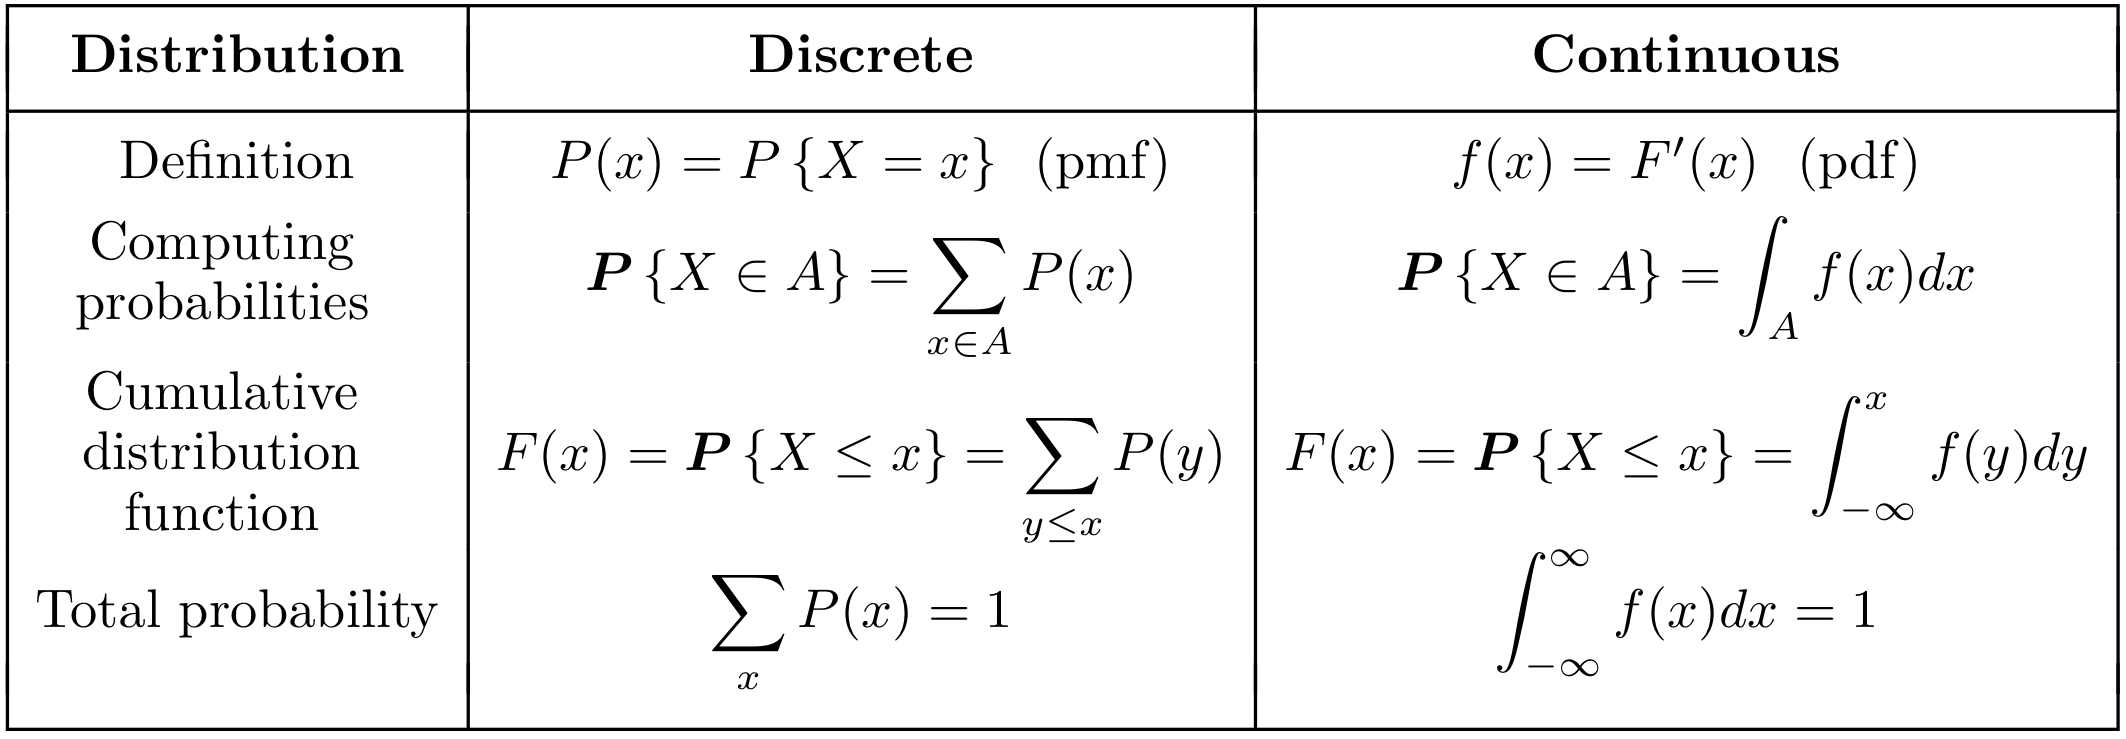
\includegraphics[width=1\linewidth]{images/pmf_cdf.jpeg}
\end{center}
\end{figure}

\begin{figure}[h]
\begin{center}
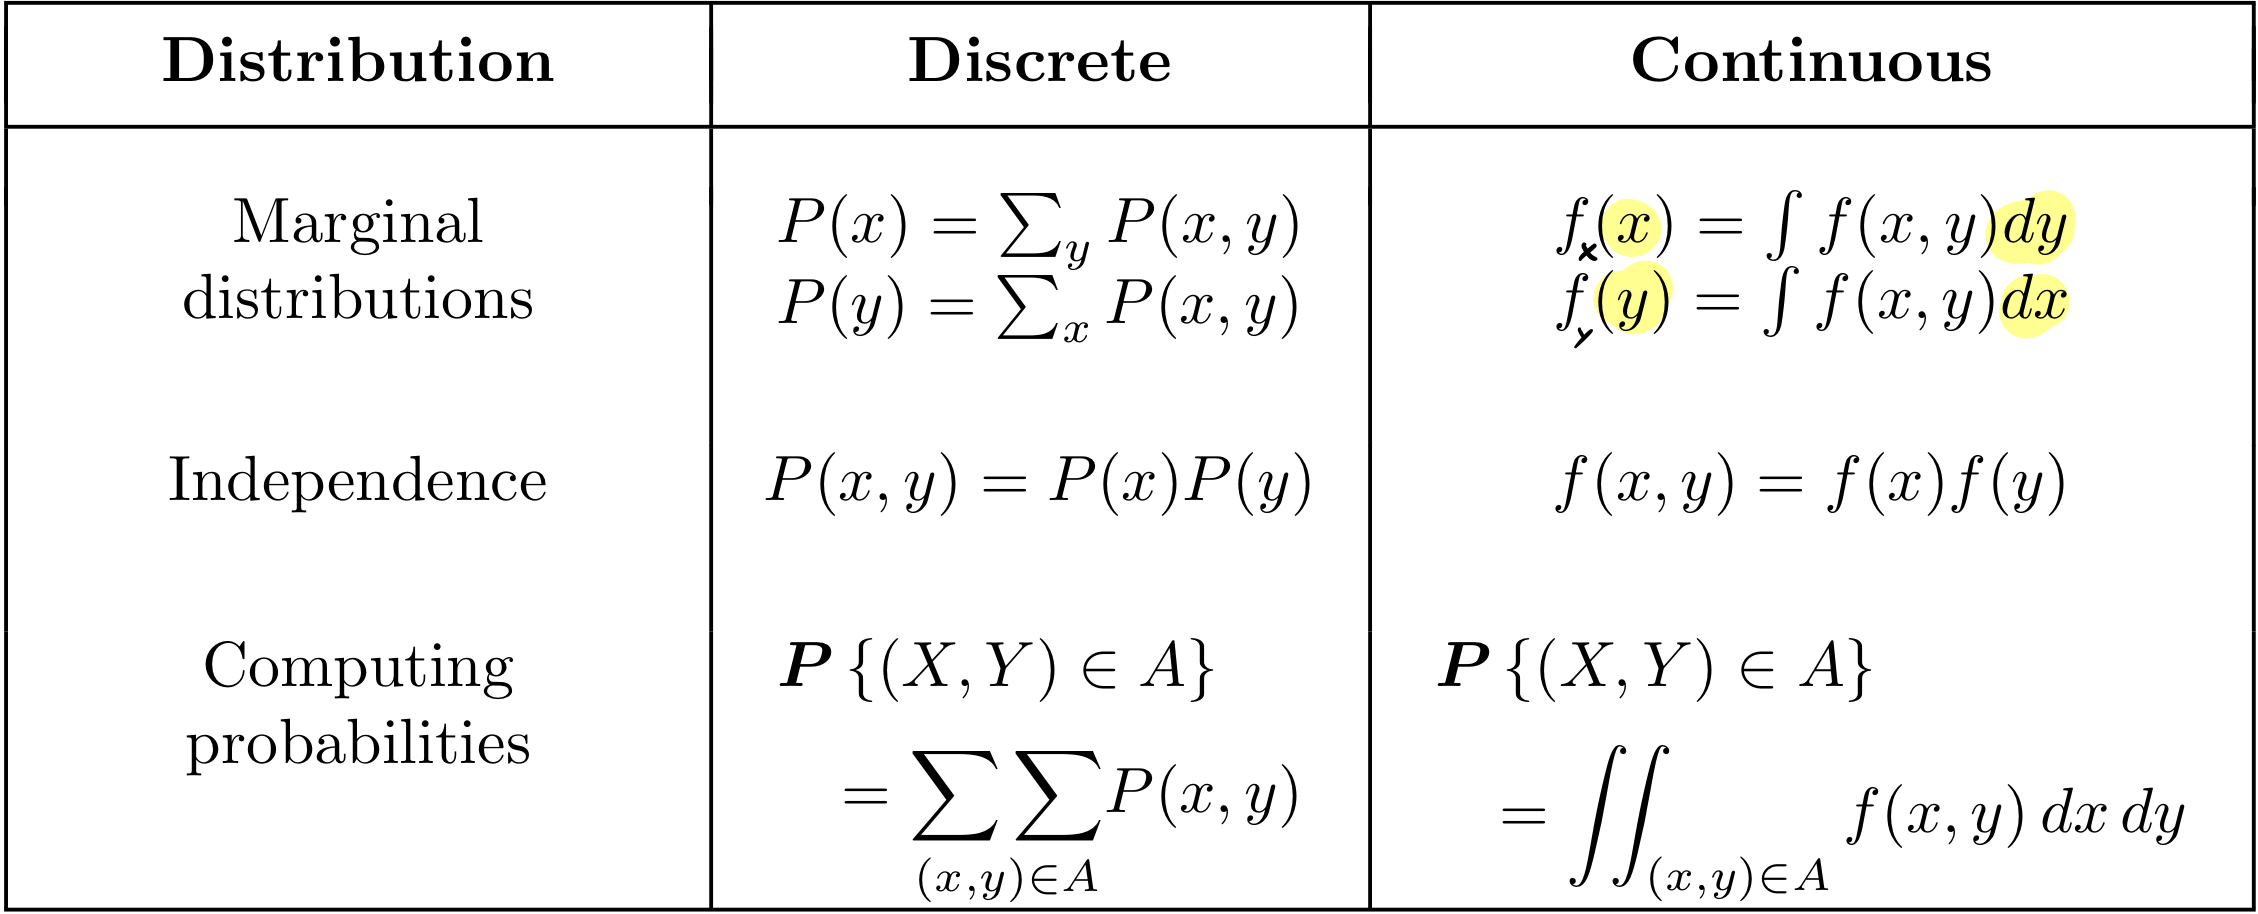
\includegraphics[width=1\linewidth]{images/marginal.jpeg}
\end{center}
\end{figure}

\textbf{Probabilità Condizionata}
\begin{itemize}
    \item \textit{Caso Discreto}
    $$P_{y|x}(y|x) = \frac{P_{xy}(x,y)}{P_{xx}(x)}$$
    $$P_{x|y}(x|y) = \frac{P_{xy}(x,y)}{P_{yy}(y)}$$
    Se $X$ e $Y$ sono indipendenti, allora
    $$P_{y|x}(y|x) = \frac{P_{xy}(x,y)}{P_{xx}(x)} = \frac{P_{xx}(x) \cdot P_{yy}(y)}{P_{xx}(x)} = P_{yy}(y)$$
    \item \textit{Caso Continuo}
    $$f_{y|x}(y|x) = \frac{f_{xy}(x,y)}{f_{xx}(x)}$$
    $$f_{x|y}(x|y) = \frac{f_{xy}(x,y)}{f_{yy}(y)}$$
    Se $X$ e $Y$ sono indipendenti, allora
    $$f_{y|x}(y|x) = \frac{f_{xy}(x,y)}{f_{xx}(x)} = \frac{f_{xx}(x) \cdot f_{yy}(y)}{f_{xx}(x)} = f_{yy}(y)$$
\end{itemize}

\begin{figure}[h]
\begin{center}
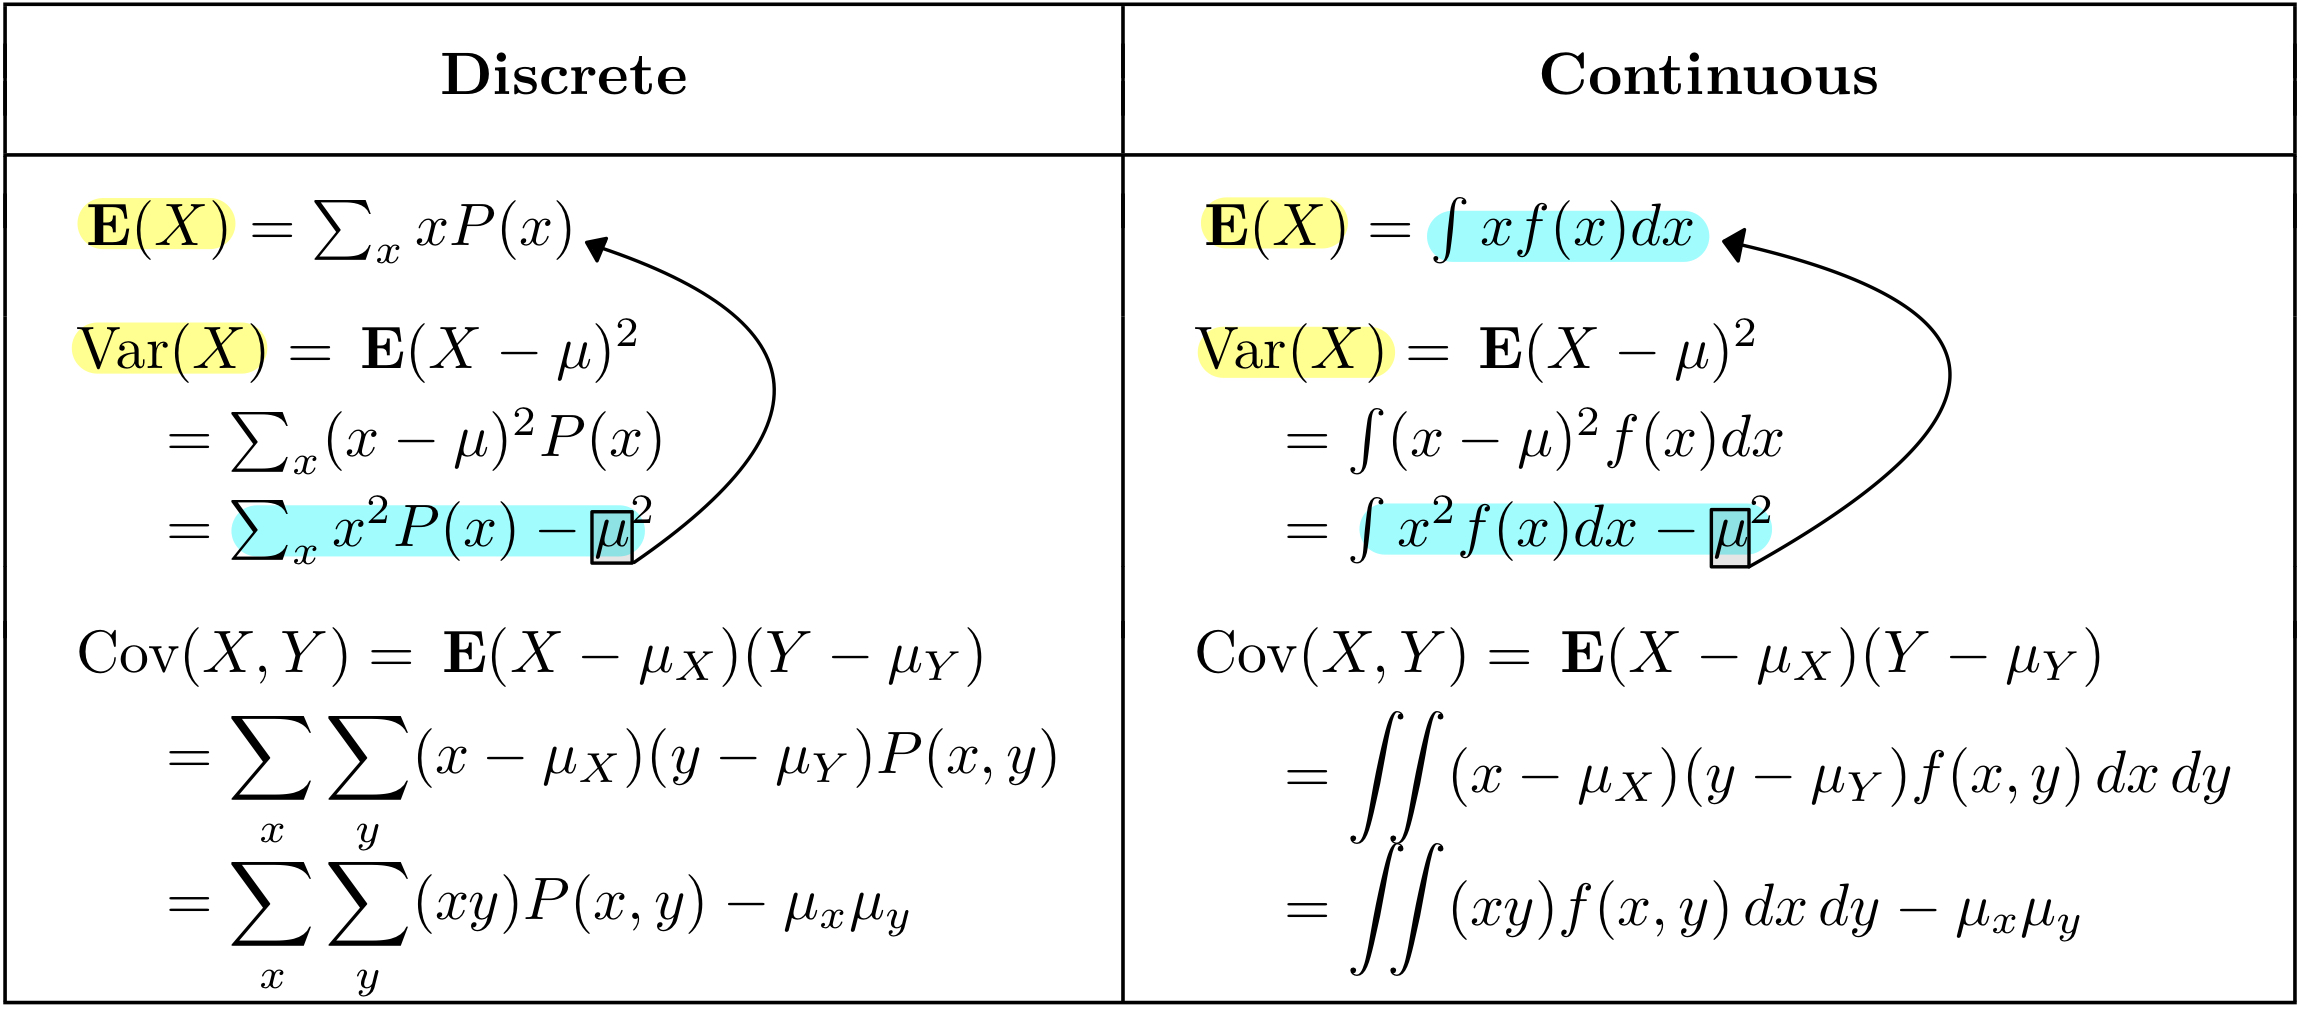
\includegraphics[width=1\linewidth]{images/e_var_cov.jpeg}
\end{center}
\end{figure}